\documentclass[a4paper,12pt]{article} 
\usepackage[T2A]{fontenc}			
\usepackage[utf8]{inputenc}			
\usepackage[english,russian]{babel}	
\usepackage{amsmath,amsfonts,amssymb,amsthm,mathrsfs,mathtools} 
\usepackage[colorlinks, linkcolor = purple, citecolor = purple]{hyperref}
\usepackage{xcolor}
\usepackage{xpatch}
\usepackage{marvosym}
\usepackage{cancel}
\usepackage{floatrow}
\usepackage{commath}
\usepackage{upgreek}
\usepackage{lipsum}
\usepackage{mhchem}
\usepackage{chemfig}
\usepackage{multirow}
\usepackage{tikz}
\usepackage{titletoc}
\usepackage{pgfplots}
\usepackage{wrapfig}
\usepackage{chngcntr}
\usepackage{makecell}
\usepackage{stackengine,graphicx}
\usepackage{cmap}
\usepackage{indentfirst}
\usepackage{tocloft}
\usepackage{setspace}
\usepackage{titlesec}
\usepackage{soul}
\usepackage[stable]{footmisc}
\usepackage{tocloft}
\usetikzlibrary{positioning}
\usepackage{caption}
\usepackage{subfig}
\pgfplotsset{width=10cm,compat=1.9}
\tikzset{>=stealth}
\usepackage[left=2cm,right=2cm,top=2cm,bottom=3cm,bindingoffset=0cm]{geometry}
%\DeclareMathOperator*{\esssup}{ess\,sup}
\DeclareMathOperator*{\tr}{tr}
\DeclareMathOperator*{\Ker}{Ker}
\DeclareMathOperator*{\Rea}{Re}
\DeclareMathOperator*{\Ima}{Im}
\DeclareFontEncoding{LS2}{}{\noaccents@}
\DeclareFontSubstitution{LS2}{stix}{m}{n}
\DeclareSymbolFont{arrows3}{LS2}{stixtt}{m}{n}
\DeclareMathSymbol{\squareulblack}{\mathord}{arrows3}{"88}
\date{\vspace{-10pt}}
\author{Дорогинин Д.В.\\
Группа Б02-825}
\title{\textbf{5.1.2. Исследование эффекта Комптона.}}


\theoremstyle{definition}
\newtheorem*{definition}{Определение}
\newtheorem{statement}{Предложение}
\newtheorem{lemma}{Лемма}
\newtheorem{theorem}{Теорема}
\newtheorem*{theorem*}{Теорема}
\newtheorem*{corollary}{Следствие}
\newtheorem*{example}{Пример}
\setcounter{tocdepth}{2}
%\renewcommand\cftsecafterpnum{\vspace{-pt}}
%\renewcommand\cftsecafterpnum{\vspace{1pt}}
\newcommand*{\eqdef}{\mathop{\overset{\mathrm{def}}{\resizebox{\widthof{\ensuremath{\mathop{\overset{\mathrm{def}}{=}}}}}{\heightof{=}}{=}}}}
\renewcommand\qedsymbol{$\squareulblack$}
\renewcommand{\cftsecleader}{\cftdotfill{\cftdotsep}}
\newfloatcommand{capbtabbox}{table}[][\FBwidth]
\newcommand{\HH}{\mathcal{H}}
\newcommand{\DD}{\mathcal{D}}
\newcommand{\LL}{\mathcal{L}}
\newcommand{\AAA}{\mathscr{A}}
\newcommand{\SpA}{\mathcal{A}}
\newcommand{\EE}{\mathcal{E}}
\newcommand{\suml}{\sum\limits_{n=1}^\infty}
\newcommand{\sumlN}{\sum\limits_{n=1}^N}
\newcommand{\sumo}{\sum\limits_{n=0}^\infty}
\newcommand{\sumoN}{\sum\limits_{n=0}^N}
\renewcommand\cftsecfont{\normalsize}
\renewcommand\cftsubsecfont{\normalsize}
\titleformat{\section}
  {\normalfont\fontsize{16}{16}\bfseries}{\thesection}{1em}{}
\def\rlwd{.5pt}
\def\crossy{\kern.5pt\def\stacktype{L}%
 \stackon[0.65ex]{%
  \stackon[1.4ex]{%
    \stackon[1.1ex]{\rule{\rlwd}{1.8ex}}{\rule{1.4ex}{\rlwd}}%
  }{\rule{0.8ex}{\rlwd}}%
 }{\rotatebox{-20}{\rule{0.8ex}{\rlwd}}}%
\kern1pt}



\newcommand{\angstrom}{\mbox{\normalfont\AA}}

\begin{document}
\maketitle
\textbf{В работе}: с помощью сцинтилляционного спектрометра исследуется энергетический спектр $\gamma$-квантов, рассеянных на графите. Определяется энергия рассеянных $\gamma$-квантов в зависимости от угла рассеяния, а также энергия покоя частиц, на которых происходит комптоновское рассеяние.
\section*{Теория}
Пусть на покоящийся электрон (энергия покоя $mc^2$) налетает $\gamma$-квант с начальной энергией $\hbar \omega_0$. После соударения электрон приобретает энергию $\gamma mc^2$ и импульс $\gamma mv$, а $\gamma$-квант рассеивается на некотрый угол $\theta$ по отношению к начальному направлению с новой энергией $\hbar \omega_1$. Из законов сохранения импульса и энергии можно получить, что разница между длинами волн падающего и рассенного $\gamma$-квантов
\begin{equation}\label{1}
\Delta \lambda = \lambda_1 - \lambda_0 = \dfrac{h}{mc} (1-\cos \theta).
\end{equation}
В наличии этой разницы и заключается эффект Комптона. Для дальнейшего применения полезно будет представить \eqref{1} в виде
\[\tag{1a}\label{1a}
\dfrac{1}{\varepsilon(\theta)} - \dfrac{1}{\varepsilon_0} = 1 - \cos \theta,
\]
где $\varepsilon_0 = E_0/mc^2$ -- начальная энергия $\gamma$-квантов в единицах $mc^2$, $\varepsilon(\theta)$ -- энергия рассеянных $\gamma$ -квантов в тех же единицах.\\
Отметим, что всё вышесказанное применительно в том случае, когда электрон свободный, что справедливо для лёгких атомов, где энергия связи не больше нескольких килоэлектрон-вольт, а чаще всего меньше, и $\gamma$-квантов с энергией в несколько десятков-сотен килоэлектрон-вольт.
\section*{Описание установки}
\begin{figure}[h]
    \subfloat{{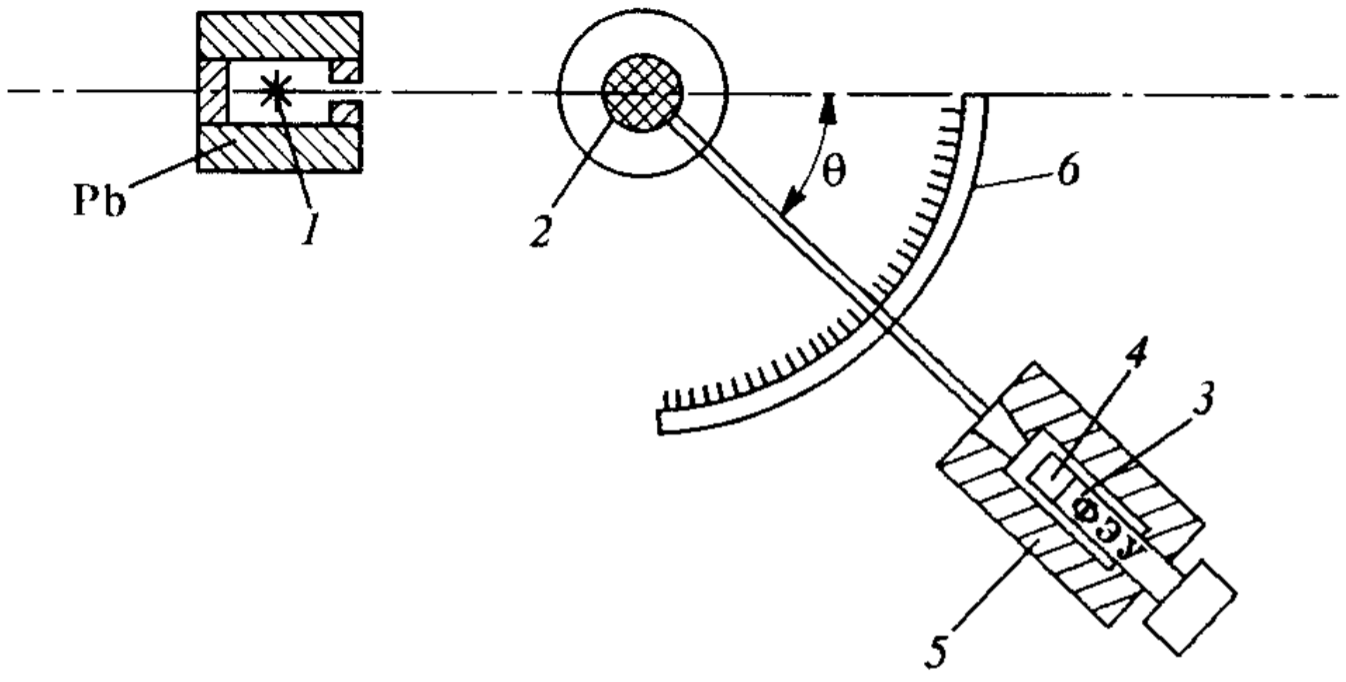
\includegraphics[width=0.5\textwidth]{1.png}}}
    \subfloat{{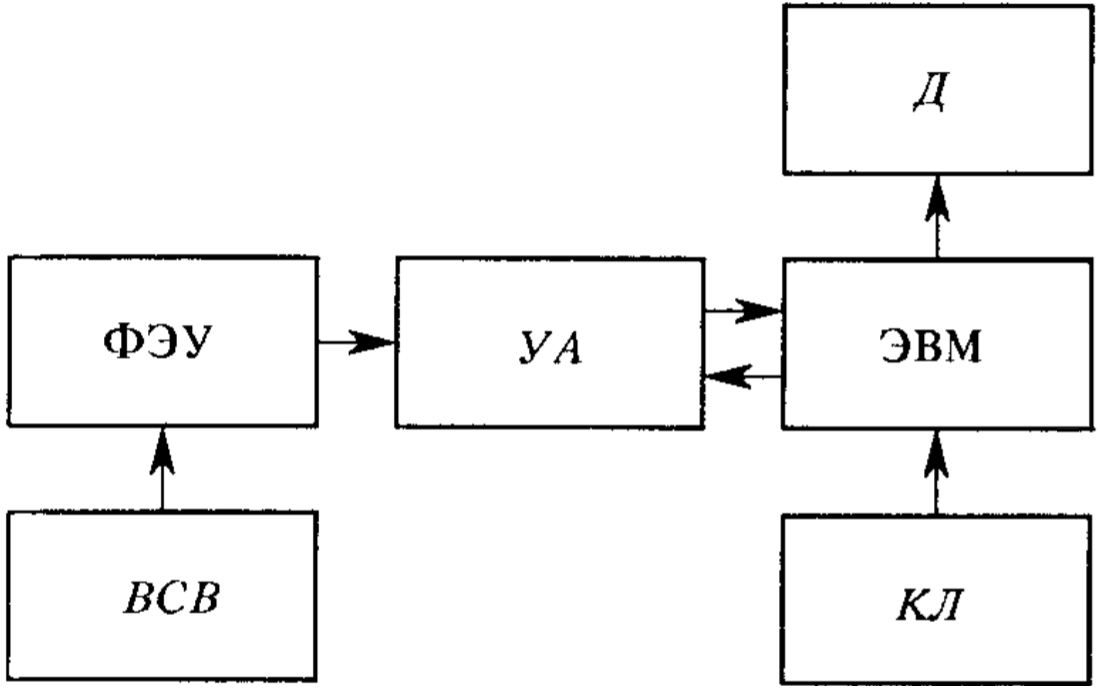
\includegraphics[width=0.5\textwidth]{2.png}}}
  \centering
  \caption{(a) Блок-схема установки по изучению рассения $\gamma$-квантов. (b) Блок-схема измерительного комплекса.}
\end{figure}
На Рис. 1а изображена блок-схема установки. Источником (1) служит $\ce{^137Cs}$, испускающий $\gamma$-лучи с энергией $662$ кэВ, который помещён в толстостенный свинцовый контейнер с коллиматором. Сформированный коллиматором узкий пучок $\gamma$-квантов попадает на графитовую мишень (2), испытывает рассеяние и регистрируется сцинтилляционным счётчиком, состоянищим из фотоэлектронного умножителя (ФЭУ) и сцинтиллятора -- выходное окно сцинтиллятора находится в оптическом контакте с фотокатодом ФЭУ. Сигналы, возникающием в аноде ФЭУ, подаются на компьютер для амплитудного анализа. Кристалл и ФЭУ расположены в светонепроницаемом блоке, укреплённого на горизонтальной штанге, которая может вместе с ним вращаться, угол поворота отсчитывается по лимбу (6). Головная часть сцинтилляционного блока закрыта свинцовым коллиматором (5), который формирует входной пучок и защищает детектор от постороннего излучения, в основном $\gamma$-квантов, проходящих через стенки защитного контейнера источника. При больших углах измерения для дополнительной защиты между контейнером и источником и детектором ставился свинцовый экран.
\begin{figure}[h]
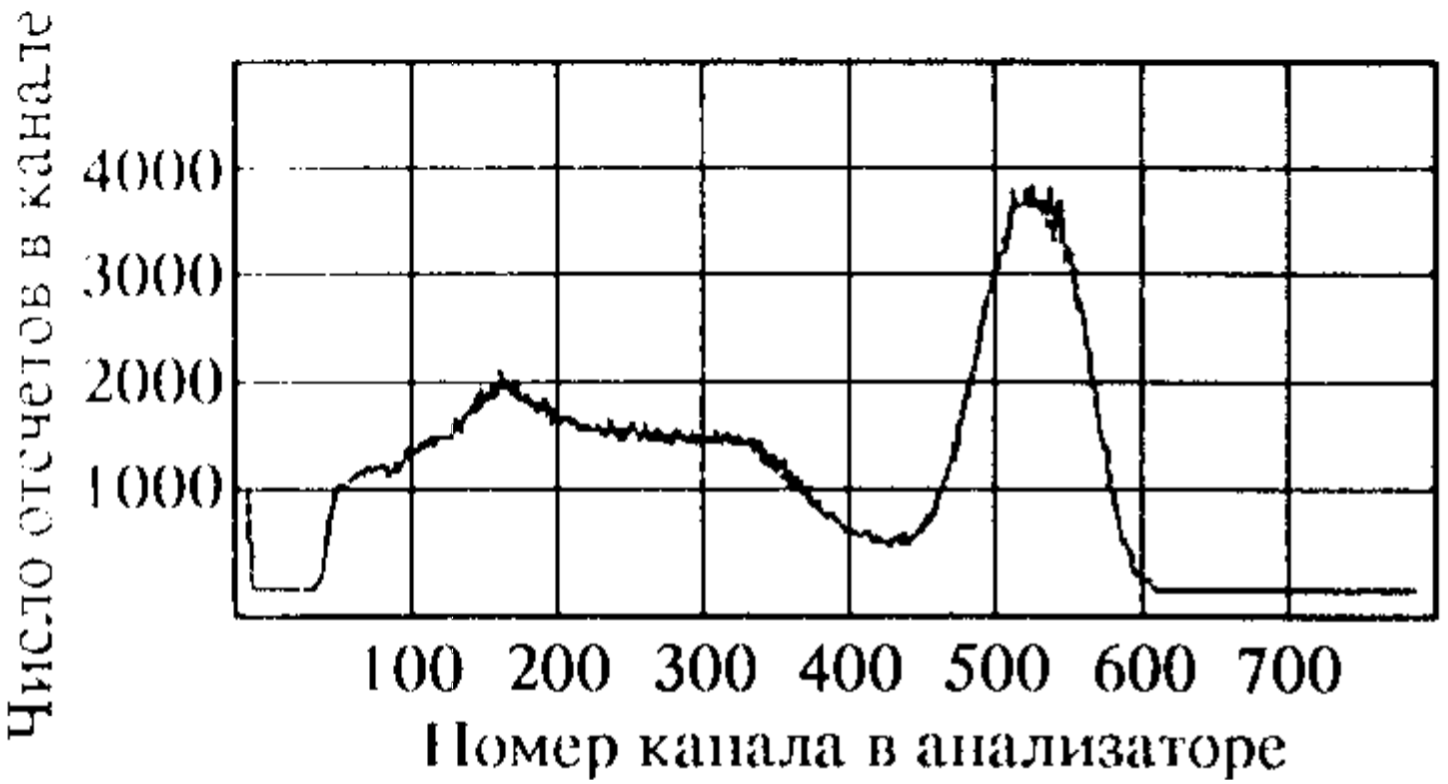
\includegraphics[width = 0.7\textwidth]{3.png}
\centering
\caption{Амплитудное распределение импульсов, возникающих в сцинтилляторе.}
\end{figure}\\
Измерительный комплекс состоит из ФЭУ, питаемого от высоковольтного выпрямителя ВСВ, усилителя-анализатора УА, являющегося входным интерфейсом компьютера ЭВМ, управляемого с клавиатуры КЛ (Рис. 1b). Информация отображается на дисплее Д. При работе ФЭУ в спектрометрическом режиме величина выходного электрического импульса пропорциональна энергии регистрируемого $\gamma$-кванта. В итоге возникает распределение электрических испульсов (Рис. 2), имеющее фотопик, положение вершины которого нас будет интересовать. Левее фотопика начинается непрерывный спектр комптоновских электронов, который сохраняется при любом угле рассеяния. Номер канала на распределении соответствует энергии регистрируемой частицы, точность его определения примерно $1\%$.
\newpage
Пусть $\varepsilon(\theta) = AN(\theta)$, $A$ -- коэффициент пропорциональность, $N(\theta)$ -- номер соответствующего канала. Тогда \eqref{1a} перепишется как
\[\tag{1b}\label{1b}
\dfrac{1}{N(\theta)} - \dfrac{1}{N(0)} = A(1-\cos \theta).\]
Отсюда можно определить энергию покоя электрона как 
\begin{equation}\label{2}
mc^2 = E_\gamma \dfrac{N(90)}{N(0) - N(90)},
\end{equation}
где $E_\gamma = E_0$ -- энергия испускаемых источником $\gamma$-квантов.
\section*{Ход работы и обработка данных}
\begin{wrapfigure}{r}{0.45\textwidth}
\vspace{-1cm}
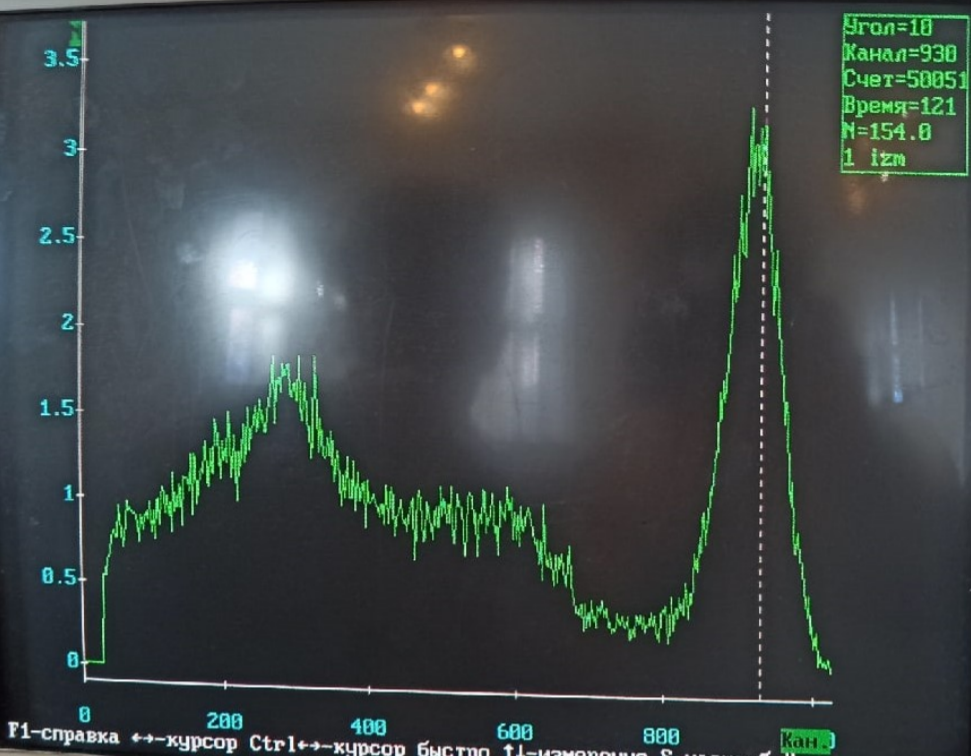
\includegraphics[width = 0.9\textwidth]{4.png}
\centering
\caption{Наблюдаемая на дисплее компьютера картина.}
\end{wrapfigure}
Устанавливая сцинтилляционный счётчик под разными углами $\theta$, произведём измерения, каждое примерно по десять минут, отмечая, какому каналу соответствует фотопик при каждом значении угла. Картина, наблюдаемая на дисплее компьютера, представлена на Рис. 3
Результаты измерений представлены в Таблице 1, как отмечалось выше, погрешнсть измерения канала -- 1\%, так как она для всех измерений больше, чем половина расстояния до соседнего возможного пика, учитывалась только она, погрешность измерения угла $\theta$ берём ценой деления лимба $\sigma_\theta = 2^\circ$.
\begin{table}[h]
\begin{tabular}{|c|c|c|c|c|c|c|c|c|c|c|c|c|c|}
\hline
$\theta$, $^\circ$ & 0   & 10  & 20  & 30  & 40  & 50  & 60  & 70  & 80  & 90  & 100 & 110 & 120 \\ \hline
$N$                & 931 & 918 & 819 & 784 & 713 & 608 & 533 & 471 & 417 & 382 & 352 & 319 & 311 \\ \hline
$\sigma_N$         & 9   & 9   & 8   & 8   & 7   & 6   & 5   & 5   & 4   & 4   & 4   & 3   & 3   \\ \hline
\end{tabular}
\centering
\caption{Результаты измерений.}
\end{table}
По этим данным постоим график зависимости $1/N(\theta)$ от $1-\cos \theta$ (Рис. 4). Здесь погрешности считали по формулам
\[\begin{array}{l}
\sigma_{1/N} = \dfrac{\sigma_N}{N^2},\\
\sigma_{1-\cos \theta} = \sin(\theta) \sigma_\theta.\\
\end{array}\]
Заметим, что во все формулы $\theta$ и $\sigma_\theta$ подставляется в радианах. Из графика по МНК получим угловой коэффициент, в соответствии с \eqref{1b} равный $A$, и точку пересечения с осью ординат, соответветствующую $1/N(0)$. Формулы расчёта (здесь $x \eqdef 1 -\cos\theta$ и $y \eqdef 1/N$):
\[\begin{array}{l l}
A = \dfrac{\langle xy \rangle - \langle x \rangle \langle y \rangle}{\langle x^2 \rangle - \langle x \rangle^2}, & \sigma_A = \dfrac{1}{\sqrt{n}}\sqrt{\dfrac{\langle y^2 \rangle - \langle y \rangle^2}{\langle x^2 \rangle - \langle x \rangle^2} - A^2},\\
\dfrac{1}{N(0)} = \langle y \rangle - A \langle x \rangle, & \sigma_{1/N(0)} = \sigma_A \sqrt{\langle x^2\rangle},\\
\end{array}\]
где $\langle \cdot \rangle$ обозначает среднее значение, $n = 13$ -- число опытов.
\begin{figure}[h]
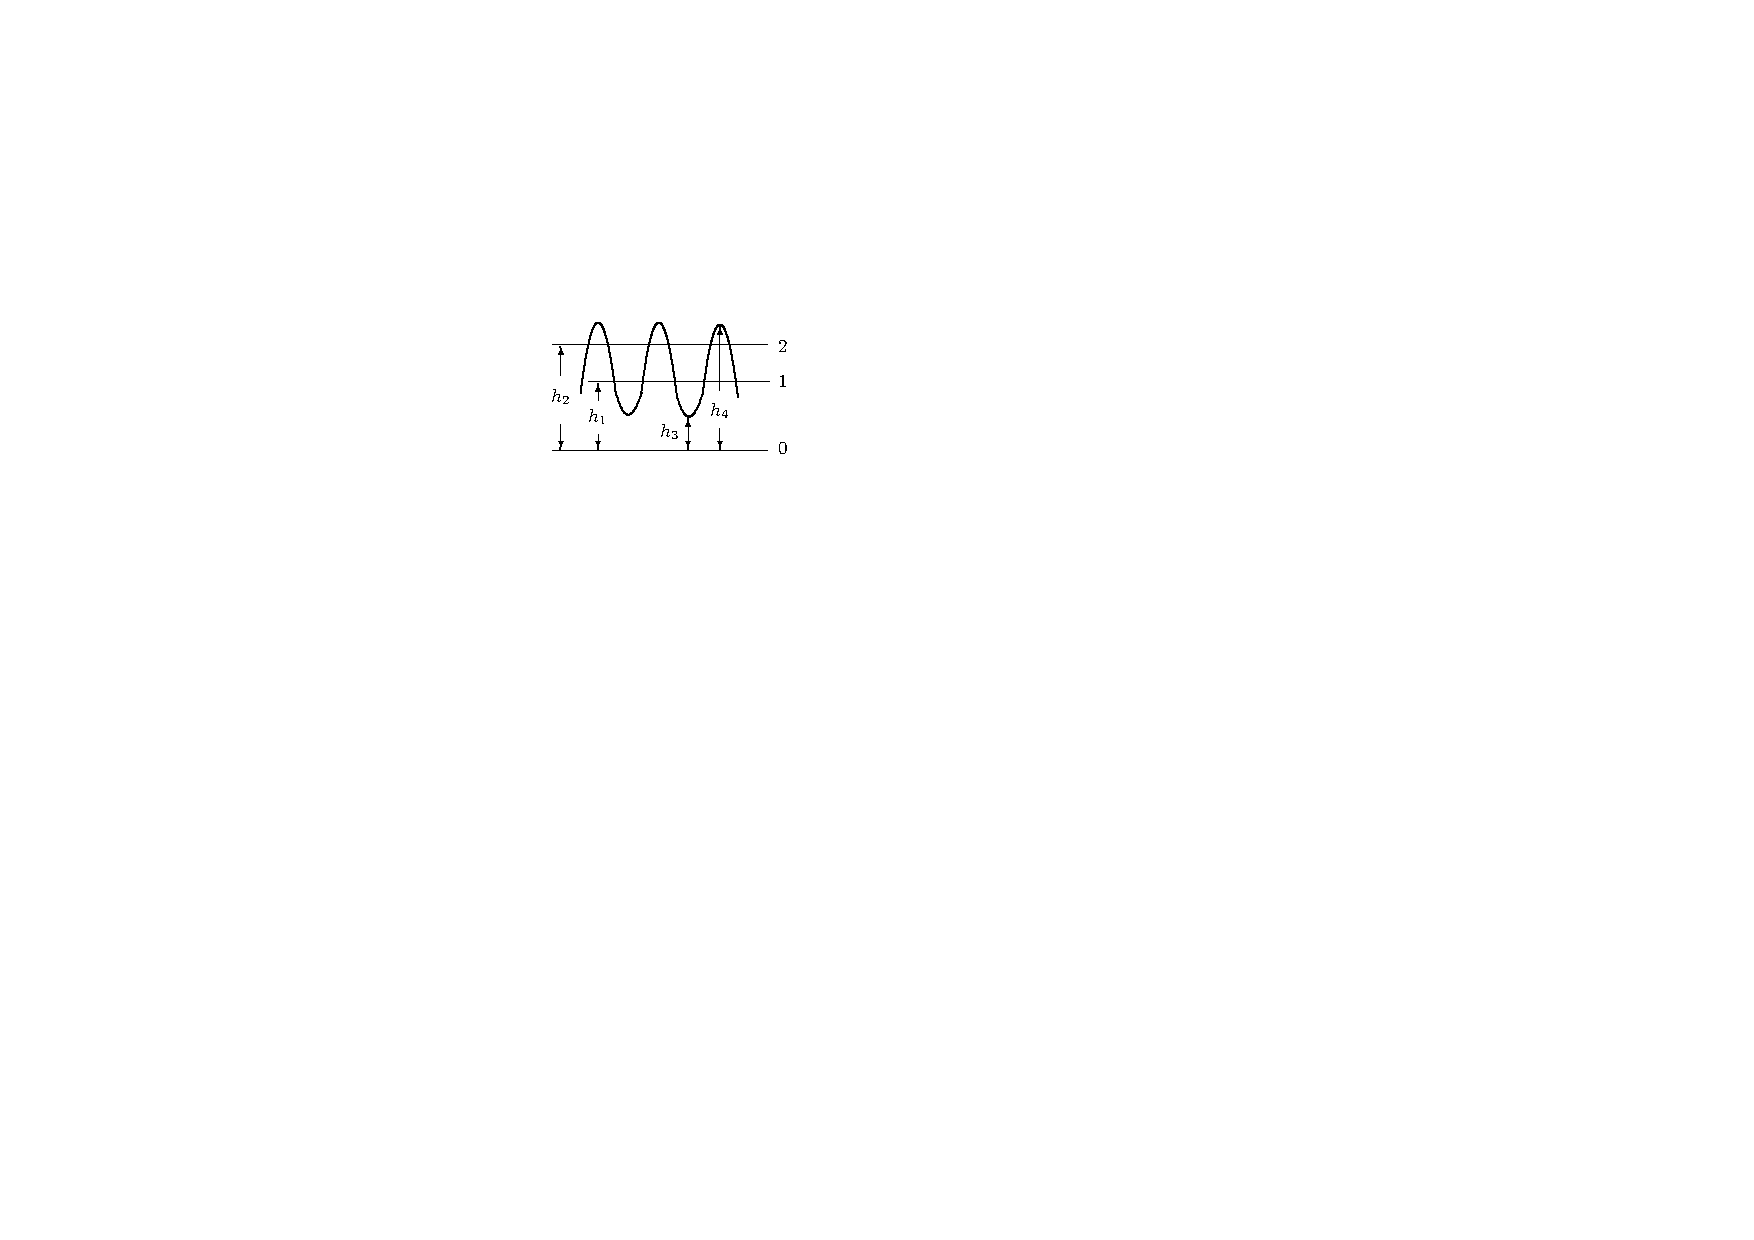
\includegraphics[width = 0.7\textwidth]{1.pdf}
\centering
\caption{График зависимости $1/N$ от $1-\cos \theta$.}
\end{figure}\\
Из аппроксимации получим <<наилучшие>> значения каналов для $\theta = 0^\circ$ и $\theta = 90^\circ$:
\[\begin{array}{l}
N_{\text{наил}}(0) = \dfrac{1}{\frac{1}{N(0)}} = 920 \pm 20,\\[12pt]
N_{\text{наил}}(90) = \dfrac{1}{\frac{1}{N(0)}+A} = 384 \pm 7,\\
\end{array}
\]
где погрешности считались по формулам
\[
\begin{array}{l}
\sigma_{N_{\text{наил}}(0)} = \dfrac{\sigma_{\frac{1}{N(0)}}}{(\frac{1}{N(0)})^2},\\[14pt]
\sigma_{N_{\text{наил}}(90)} = \dfrac{\sigma_{\frac{1}{N(0)}} + \sigma_{A}}{(\frac{1}{N(0)}+A)^2}.\\
\end{array}
\]
Наконец, по формуле \eqref{2} (для $N(0)$ и $N(90)$ брались наилучшие значения) получим энергию покоя электрона
\[mc^2 = 480 \pm 20~\text{кэВ},\]
погрешность считалась по формуле
\[\sigma_{mc^2} = \sqrt{ \left( \dfrac{\partial (mc^2)}{\partial N_{\text{наил}}(0)} \right)^2 \sigma_{N_{\text{наил}}(0)}^2 +\left( \dfrac{\partial (mc^2)}{\partial N_{\text{наил}}(90)} \right)^2 \sigma_{N_{\text{наил}}(90)}^2 }\]
Здесь использовалось, что $E_\gamma = 662~\text{кэВ}$ (значение взято из \cite{laba}). Истинная энергия покоя электрона 510 кэВ лежит в двух сигмах от полученного результата.
\section*{Заключение}
В ходе работы было исследовано рассеяние $\gamma$-квантов на графите, подтверждена теоретическая формула для распределения энергии $\gamma$-квантов по углам рассеяния, а также как следствие посчитана энергия покоя электрона $mc^2 = 480 \pm 20 ~\text{кэВ}$.
\begin{thebibliography}{9}
\bibitem{laba} 
Игошин Ф.Ф., Самарский Ю.А., Ципенюк Ю.М. 
\textit{Лабораторный практикум по общей физике: Учеб. пособие для вузов. Т. 3 Квантовая физика}. 
М.: Физматкнига, 2005.
\end{thebibliography}
\end{document}